\section{Math-Manipulator}
    \subsection{What did I do?}
        \begin{frame}
            \frametitle{What is Math-Manipulator?}

            \hspace{-2em}
            \makebox[\textwidth][c]{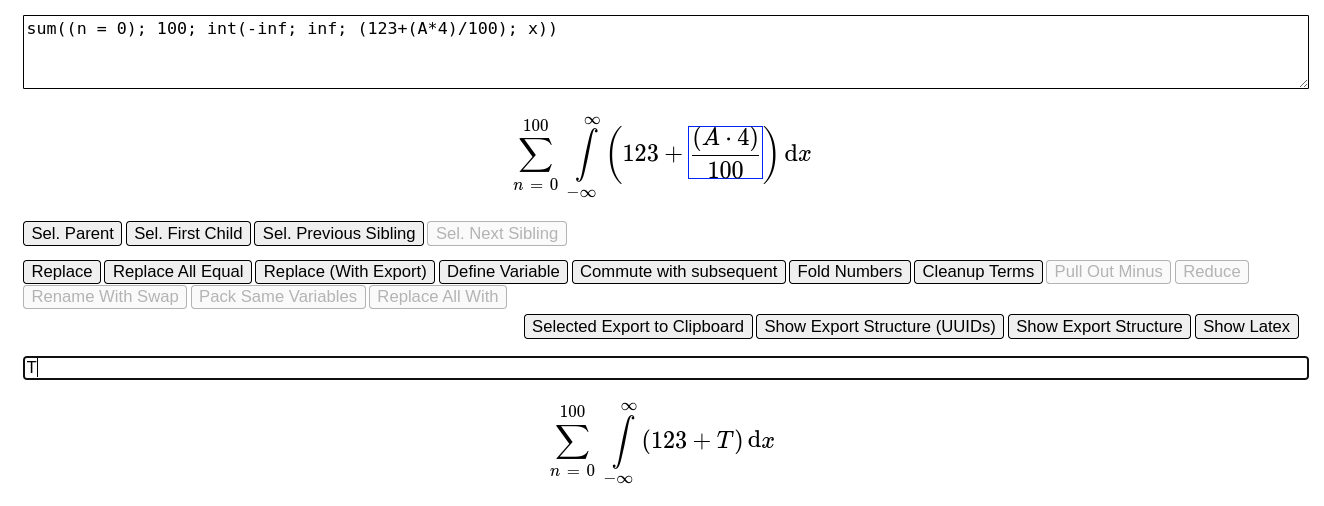
\includegraphics[width=0.9\textwidth]{main-content/math-manipulator/usage-example.png}}
            
            \blankfootnote{Math-Manipulator \cite{selfMathManipulator}}
        \end{frame}

        \note[enumerate]{
            \item I wrote a custom tool that should help with the process of doing math paper-like, but with the help of computers
            \item Features/Properties
            \begin{itemize}
                \item Relatively smart initial text-input
                \begin{itemize}
                    \item Omit implied multiplication
                    \item Omit implied zeros
                    \item Parameter autoboxing
                    \item Bracket culling
                    \item $\rightarrow$ Way less stringent as e.g. input to many Computer-Algebra-Systems requires
                \end{itemize}
                \item Once initial input is set, operations with mouse
                \begin{itemize}
                    \item Rename, Pack, Move elements with mouse interactions
                    \item Execute operator-specific operations (distribute, delta/qm-op stuff)
                \end{itemize}
                \item Many pre-defined Functions/Symbols
                \item Automatic Macro and Variable system
                \item In-Browser Help with interactive Playground
            \end{itemize}
        }
        

    \subsection{How can you use it}
        \begin{frame}
            \frametitle{In the Browser}

            \begin{itemize}
                \item Available open-source on GitHub
                \item Self-hosting possible
                \item Hosted version available in every modern browser
            \end{itemize}

            \vspace{1em}

            \begin{block}{Available here}
                \href{https://jonas-kell.github.io/math-manipulator/}{https://jonas-kell.github.io/math-manipulator/}
            \end{block}

            % notes 
            \onslide % on all slides of frame
            \note[item] {
                Source code available
            }
            \note[item] {
                (Relatively) easily extensible, tutorial and issues available
            }
            \note[item] {
                Instantly usable, offline and online
            }
        \end{frame}
    
        \begin{frame}
            \frametitle{Usage as VS-Code Extension}

            \begin{itemize}
                \item Offline-Use after installed once
                \item Store progress in files
                \item Directly integrated in powerful IDE, and with that version control
            \end{itemize}

            \vspace{1em}

            \begin{alertblock}{Note}
                Do not allow a spellchecker to run on the file, it will break everything performance-wise
            \end{alertblock}

            % notes 
            \onslide % on all slides of frame
            \note[item] {
                For more serious use, integrated in the code-editor VS-Code as an Extension
            }
            \note[item] {
                Allows for all features, but includes 
                \begin{itemize}
                    \item Offline use out of the box
                    \item Storage of files (with that version control)
                    \item Multiple parallel projects 
                \end{itemize}
            }
            \note[item] {
                Has already taken entry into my personal workflow by now
                \begin{itemize}
                    \item Probably I will never make back my WHOLE time-investment
                    \item But I already saved hours upon hours when I noticed sign mistakes, symmetry issues or similar in calculations I did with it
                \end{itemize}
            }
        \end{frame}

    \subsection{Interactive Demonstration}

        \begin{frame}
            \frametitle{Demo Problems from before}
                
            \makebox[0.9\textwidth][c]{
                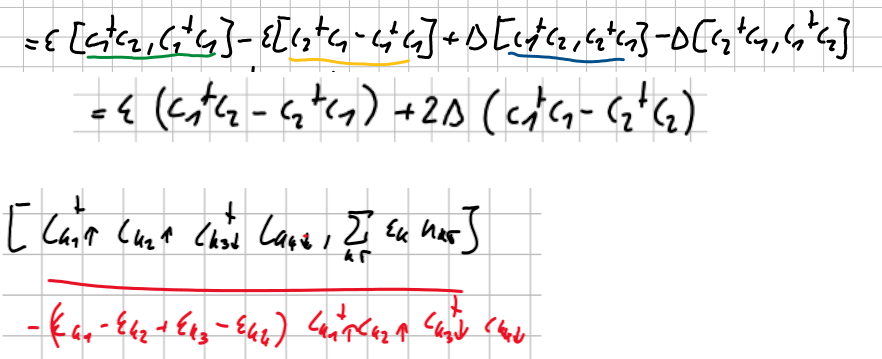
\includegraphics[width=.8\textwidth]{./math-manipulator-calculations/demo-problems.png}
            }

        \end{frame}

        \note[enumerate]{
            \item Go to Demo in VS-Code folder math-manipulator-calculations in the presentation subfolder
            \item Think of disabling spellchecker
            \item Think to first split deltas before evaluating !!!!!!
            \item Macros and other optimizations are possible, but not really necessary
            \item Input for simple demo: distribute, cleanup, order op string, \\
                \texttt{(x+y)(4*x -z+y )(-z + 1+ x)}
            \item Input for simple operators: \\
                \texttt{fc("" l)fa("" l) ;|; fc("" l)fa("" m) ;|; fc("" 1)fa("" 2) ;|; fa("" 2)fc("" 2);|; fc("" 1)fa("" 1)fc("" 3)fa("" 3)fa("" 2)fc("" 1)}
        }

        \begin{frame}[t]
            \frametitle{Usage for the Practical Training}
            
            \vspace{-1em}
            \hspace{-2em}
            \makebox[0.9\textwidth][c]{
                \includegraphics[page=3,width=.55\textwidth]{./main-content/paper/V_interaction_picture.pdf}
            }
            \hspace{-2em}
            \makebox[0.9\textwidth][c]{
                \includegraphics[page=4,width=.76\textwidth]{./main-content/paper/V_interaction_picture.pdf}
            }

            % notes 
            \onslide % on all slides of frame
            \note[item] {
                Go to Demo in VS-Code submodule mm-calculations. 
            }
            \note[item] {
                Think of disabling spellchecker
            }
            \note[item] {
                Show process of how V is calculated
            }
            \note[item] {
                Story: at the end at first result was no longer symmetrical in up and down, but it should have been. Mistake was in the very first input. But because of the upfornt configuration (and in my case programming) effort, re-calculating the endresult took 20min instead of one week
            }
        \end{frame}